\section{Common Hardware Implementation\label{sec:common_hardware_implementation}}

In order to deliver high quality modules suitable for use in the vehicle, the module electronics were all implemented on custom designed two-layer printed circuit boards. Since the project budget could only afford the manufacture of a single iteration of prototype boards, a great deal of time was spent revising both the schematics and board layouts of all four modules to fix as many issues before sending them out for manufacture.

\nomenclature{PCB}{Printed Circuit Board}

\subsection{Base System Hardware\label{sec:base_system_hardware}}

All four modules are implemented on custom printed circuit boards (PCBs), and utilize a common base platform consisting of a microcontroller, a power supply, status leds, and JTAG programming header. Additionally, the telemetry, braking, and transmission and engine control modules utilize a special sealed 23-pin connector header.

Table \ref{tab:common_module_components} lists the major non-generic components that were specified as the common base for each module. An emph{AT90CAN128} micro-controller from Atmel was chosen for several reasons. We considered several simple, low cost microcontrollers specifically for automotive use as they are typically configured with the features we need, specifically, we wanted a microcontroller with:

\begin{itemize}
  \item a \unit{5}{\volt} power supply,
  \item integrated CANBus periferal,
  \item a large amount of on-chip RAM and ROM,
  \item in-circuit debugging and programming capabilities, and
  \item a flexible and cross-platform toolchain, ideally using GNU tools like gcc.
\end{itemize}

We considered the use of a 16-bit microcontroller, but felt it would be overkill for our system. The 8-bit AT90CAN128 met our requirements very well, and we had the additional benefit of already being somewhat familiar with the Atmel platform. The AT90CAN series runs off of a \unit{5}{\volt} power supply, has integrated CANBus, in addition to lots of other periferals \cite{AT90CAN}. The AT90CAN128 provides \unit{128}{\kilo\byte} ROM, however only \unit{4}{\kilo\byte} of RAM. We felt this would however suffice. The AT90CAN also supports a JTAG debugging interface, and there exists a very well developed open-source toolchain and standard c library, both of which will be described further in Sec. \ref{sec:common_software_implementation}.

\begin{table}[H]
	\caption{Common module components.}
	\label{tab:common_module_components}
	\centering
	\begin{tabular}{|c|c|c|}
		\hline 
		Part & Manufacturer & Part Number\tabularnewline 
		\hline \hline
		CAN Bus Transceiver & Microchip & MCP2551\tabularnewline \hline
		Microcontroller & Atmel & AT90CAN128\tabularnewline \hline
		Voltage Regulator & Linear Technology & LT1129CST5\tabularnewline		
		\hline
	\end{tabular}
\end{table}

\subsection{Inter-module Communication\label{sec:inter_module_communication}}

\nomenclature{CAN}{Controller Area Network}

All electronic systems on the vehicle communicate over a two-wire \emph{Controller Area Network} (CAN) bus operating at 1 MBit/s. Each system module has a Microchip-brand MCP2551 CAN transceiver IC for connecting their local micro-controller to the bus, and all modules are capable of being a termination point for the bus \cite{MCP2551}. The CAN transceiver electrically interfaces the microcontroller to the physical bus.

\subsection{Linear Regulator}

The LT1129 from Linear Technology was chosen as the \unit{5}{\volt} regulator because of several features it offers. The device is capable of supplying up to \unit{700}{\milli\ampere}, requires only a single \unit{3.3}{\micro\farad} output capacitor, accepts input voltages up to \unit{30}{\volt}, and has built-in thermal limiting \cite{LTC1129}.

\subsection{PCB Layout and CAD Design}

Schematic capture and PCB layout were both done using the free version of EagleCAD. Schematics and PCB layouts can be seen in Appendix \ref{cha:attached_dvd}. All four modules were layed out as two-layer PCBs with a groud plane on the bottom, and a VCC plane (\unit{+5}{\volt}) on the top. This aided routing, and reduced the possibility of ground loops since any connection to ground was as short as possible. For comparison with other figures showing the design and construction process of the modules, Fig.\ \ref{fig:driver_interface_layout} shows the board layout exported from Eagle CAD of the Telemetry module board. Layouts of the other three modules are available in Sec.\ \ref{cha:attached_dvd}. Where possible, surface mount components were selected to reduce the number of drills required in the PCB (and hence the cost).

\begin{figure}[h]
  \centering
  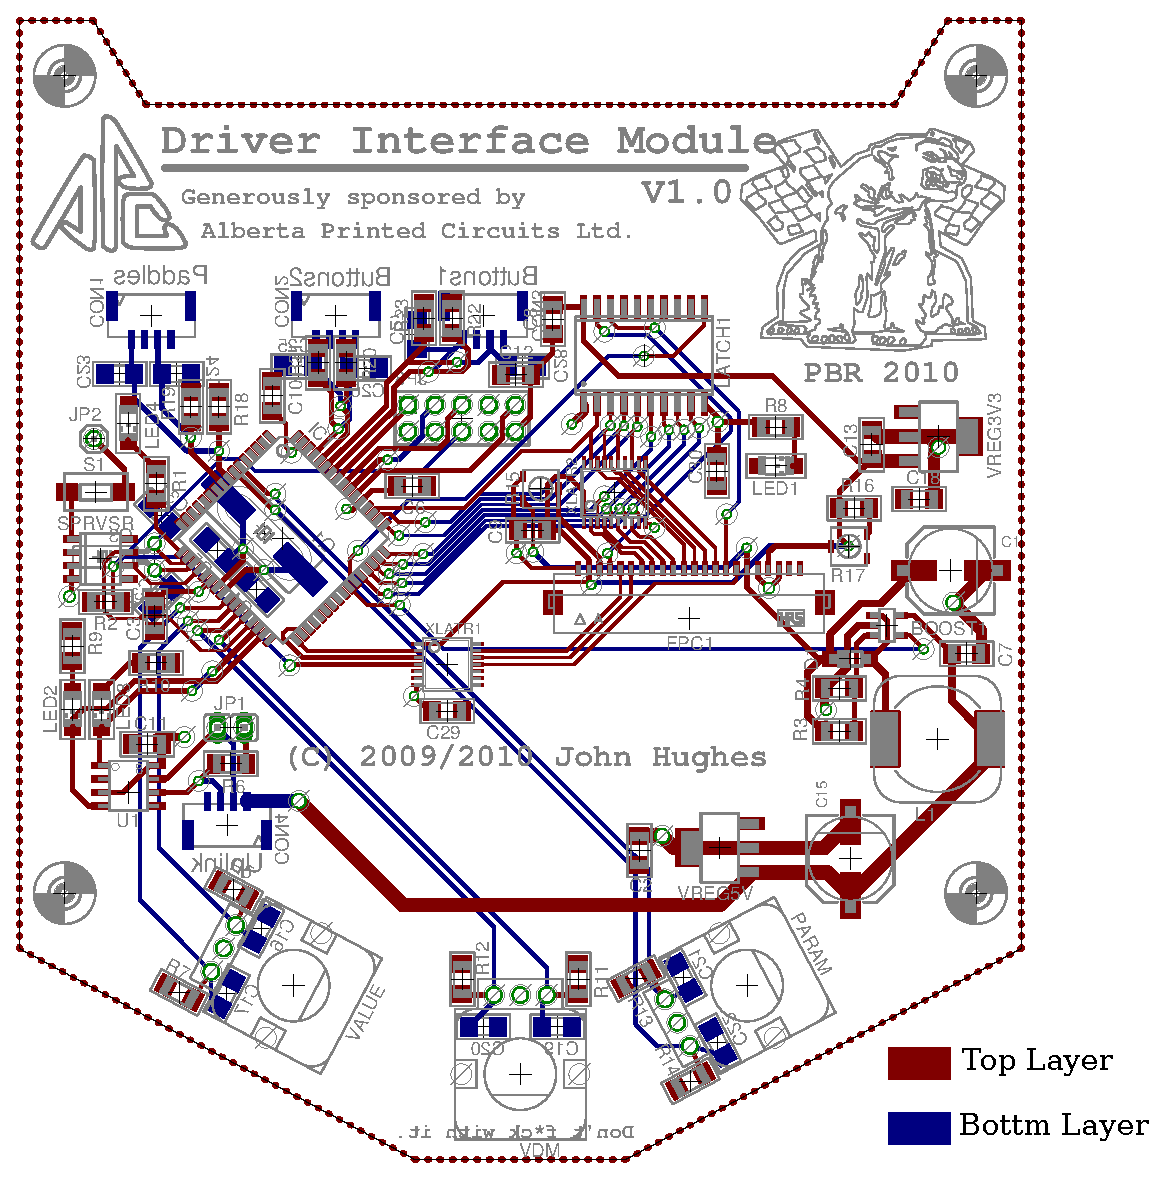
\includegraphics[width=3.5in,keepaspectratio]{implementation/figures/driver_interface_layout.eps}
  \caption{Board layout for the Telemetry module, exported from Eagle CAD.}
  \label{fig:driver_interface_layout}
\end{figure}

\subsection{Module Construction}

The printed circuit boards were manufactured by Alberta Printed Circuit (APCircuits), Ltd., who kindly sponsored the project. From the PCB layouts created in Eagle CAD, industry-standard GERBER-format files were generated and sent electronically to APCircuits. Figure \ref{fig:empty_pcbs} shows a photograph of the four empty PCBs after they were manufactured.

All four modules were populated and soldered by hand. Counter-intuitively, we found soldering the surface mount components with many leads to be easier than their through-hole counterparts. Initially we attempted to use paste stencils laser-cut out of mylar to apply the solder, in a process similar to that used in industry, however we found that for the relative incomplexity of our PCBs this was not of great aide. In the final manufacturing process, several steps were taken to populate each module:

\begin{enumerate}
  \item Once the circuit boards had arrived from manufacture, simple electrical tests were made to validate the construction: point to point checks of the ground and VCC planes were checked for continuity.
  \item An alchol-based circuit board cleaner was used to clean the surface of the boards of any contaminants.
  \item Solder paste was applied using a syringe individually to the large pads of resistors and capacitors, and in a thin strip across a line of smaller pads for the larger components.
  \item Individual components were placed on the pads with tweezers. The previously applied solder paste served as a slight adhesive.
  \item The entire board was placed in a toaster oven for approximately 7 minutes. Two-minute warm up and cool down periods were used before and after a 3 minute maximum tempurature reflow phase. The warm-up period served to evaporate the solvents in the solder paste, while the gradual cool down was performed to avoid thermal shock.
\end{enumerate}

\begin{figure}[h]
 \centering
 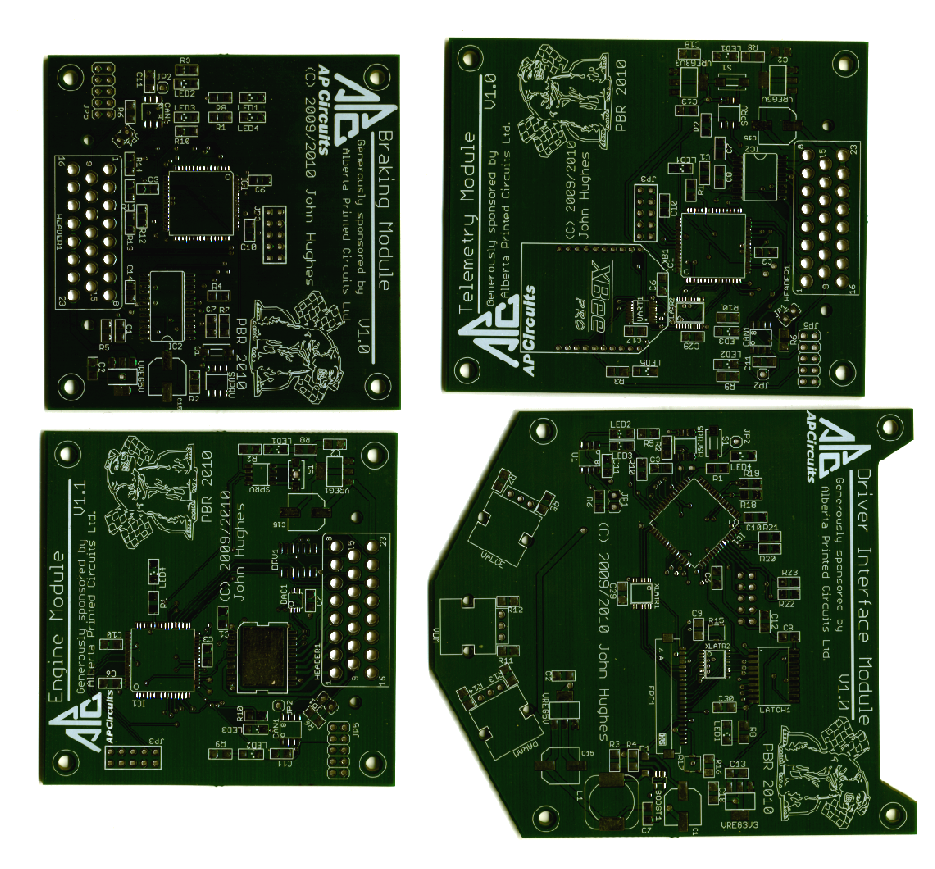
\includegraphics[width=5in,keepaspectratio]{implementation/figures/empty_pcbs.eps}
 \caption[Empty circuit boards after manufacturing.]{Empty circuit boards after manufacturing. Clockwise: Braking module, Telemetry module, Driver Interface module, and Engine and Transmission module}
 \label{fig:empty_pcbs}
\end{figure}

Color photographs of each completed module are shown in the relevant sections discussing them.